\section{Introduction}
% Paragraph 1: introduction to AES and XAS/AES and what are they needed for. if possible, find a combination of the two to explan that this is a more powerful tool to study the electronic structure


X-ray absorption and Auger spectroscopies are powerful tools to study the electronic structure and the nearest environment of atoms in \denis{dilute or condensed phases. Applied to liquids, these methods allowed collecting the response of a specific element irradiated by x-rays, and gave new insight into the determination of the structure of simple aqueous solutions} \citep{Pokapanich09:7264}, and to the mechanisms of radiation damage \citep{ONeill02:329,Carugo05:213,Stumpf16:237}. The absorption of an \denis{energetic photon} leads to the creation of core-excited or core-ionized states, \denis{followed on a very short timescale by different types of electronic decays.} \denis{For an atom, the relaxation of these states occurs via ultrafast radiative or non-radiative processes. However, if the initially excited or ionized element is embedded in an environment, delocalized relaxation mechanisms such as interatomic Coulombic decay (ICD) and related processes \citep{Pokapanich09:7264,Pokapanich11:13430,Stumpf16:237,unger17:708} are possible}.

\denis{It has been rather well described in the case of atoms and molecules that the character of the core-ionized states strongly influences the decay processes (REFS) \citep{stoychev08:074307,Demekhin08:043421,Demekhin09:104303,Ouchi11:053415,Miteva14:164303,Miteva14:064307}}\denis{{\textbf{What do you mean by character? Configuration?}}}
%The course of a decay cascade depends on the character of the initially populated states.
%This has been well understood in atoms and molecules in gas phase (REFS) \citep{stoychev08:074307,Demekhin08:043421,Demekhin09:104303,Ouchi11:053415,Miteva14:164303,Miteva14:064307}. 
\\
\textbf{Starting from a neutral species, the direct core ionization process, followed by an Auger decay (see Fig.\ \ref{fg:auger}), leads to the population of doubly ionized final states localized on the initially ionized unit \citep{stoychev08:074307,Demekhin08:043421,Demekhin09:104303,Ouchi11:053415}. \denis{Auger lines can come from delocalized states. I think that the corresponding matrix element reflects the overlap of the different orbitals involved in the process. This must be changed from my point of view. I wait for your comments first} Auger processes in rare gas clusters have been also investigated \citep{Wurth93:6697} (REFS). The normal Auger decay process in these systems proceeds similarly to that in atoms or molecules. However, in the case of a core excited state, the resonant Auger process competes with the process of delocalization of the excited electron in clusters \citep{Bjorneholm95:3017}. If the initially core excited electron delocalizes within the lifetime of the core hole, then normal instead of resonant Auger decay is observed \citep{Bjorneholm95:3017}. 
}

In a solution, the electronic decays initiated by the x-ray absorption are different compared to those in rare gas clusters \denis{due to the nature of the bonds} and due to shorter interatomic distances \denis{leading to} stronger interactions. In particular, the solvent molecules have two effects -- first, they affect the excited \citep{miteva16:16671} or ionized states of the ion \denis{\textbf{(what do you mean by "they affect"? You talk about the energy levels?)}}and second, they can participate in the decay processes, leading to the population of delocalized final states, and thus ionizing the surrounding environment \citep{Pokapanich09:7264,Pokapanich11:13430,Stumpf16:237}.\textbf{ Moreover, the process of delocalization of the initially excited electron also occurs in aqueous solutions \citep{Nordlund07:217406,Ottosson11:13489}.}
%Moreover, the process of delocalization of the initially excited electron is not specific to rare gas clusters, but it also occurs in aqueous solutions \citep{Nordlund07:217406,Ottosson11:13489}. 
In the case of pure water, the rate of delocalization of the oxygen 1s excited electron takes place on a femtosecond to sub-femtosecond time scale depending on the photon energy, \denis{i.e. from pre- to post-edge excitation}, being thus much faster than the 6\,fs of the O1s core-hole lifetime\citep{Nordlund07:217406}. Working at higher photon energies \denis{means that deeper core-levels can be reached}. The lifetimes of the corresponding core-ionized states become even shorter \citep{ceolin17} and thus, it is even more imperative\textbf{ (Challenging?) }to reveal whether the delocalization of the core-excited electron occurs within the lifetime of the core-hole.


The aim of this work is to elucidate the nature of the states populated upon hard x-ray irradiation of solvated ions, \denis{to describe the states populated after the main non-radiative electronic relaxation chanel of the core-hole}, and furthermore, to understand \denis{how} possible electron delocalization \denis {processes occurring during the core-hole lifetime} influences the electronic decays. To this end, we used resonant and normal Auger spectroscopies together with x-ray absorption spectroscopy to investigate aqueous potassium chloride solution at the K-edges of both \ki~and \cli ions. In particular, we demonstrate experimentally that at photon energies below the K-edges of the solvated ions, localized core-excited states are populated \denis{despite not being clearly visible on the absorption spectra}. Moreover, we observe that although the \ki~and \cli~ions are isoelectronic, they have different fingerprints in the resonant Auger spectra. With the aid of high-level {\it ab initio} calculations of the initial and final states of the resonant Auger process of both the bare ions and their microsolvated clusters, we demonstrate that these differences are a result of the different electronic structures of the two ions, thus confirming that the XAS/AES technique is a sensitive probe of the electronic structure of solutions. In addition, the core-excited states undergo a decay \denis{on a timescale of about 1\,fs which corresponds to the 1s core-hole lifetime of chloride and potassium ions. For both species}, \textbf{there is a competition between resonant Auger decay and delocalization of the excited electron}. Using the core-hole clock method (REFS\denis{Olle, Faris}), we show that in \ki~, delocalization at the pre-edge is weak, whereas in the case of \cli, due to the energetic proximity of the core-excited states very close to the K-edge, the rate of delocalization is of the same order as that of the resonant Auger process. 

\begin{figure}
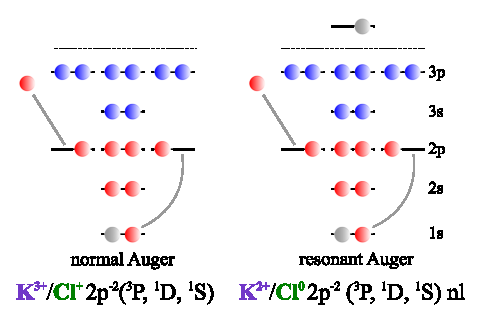
\includegraphics{figures/auger_process.eps}
\caption{Schematic representation of the normal and resonant Auger processes.}
\label{fg:auger}
\end{figure}